\documentclass[12pt]{book} % Default is book 12 pt regular A4 based on setting file
% Default regular A4, based on setting file 
\usepackage[paper = a4paper,         %To be shrunk to 80% when printed
			twoside,                 %Two-side mode, switches margins on
			bindingoffset = 2mm,     %Offset for binding side of page
			hmargin = 25mm,          %Left and right margin
            vmargin = 25mm,          %Top and bottom margin
			dvipdfm]
			{geometry}

%****************************************************************
% Note: Make all your adjustments in here in preamble and macros 
%****************************************************************
%
% Include all packages
%
%!TEX root = ./thesis.tex 
%%%%%%%%%%%%%%%%%% % Font settings %%%%%%%%%%%%%%%%%%%%% 
\usepackage[osf]{newpxtext} % Palatino font with old-style figures
\linespread{1.05}
\usepackage[T1,euler-digits]{eulervm} % Euler-VM fonts for maths 
\usepackage[scaled]{beramono}   % typewriter font
\usepackage[T1]{fontenc}	    % Activate Type 1 fonts 
\usepackage[utf8]{inputenc}     % We want æøå 
\usepackage{sectsty}            % Change section and chapter header 
\usepackage{textcomp}
\usepackage{anyfontsize}
\usepackage[protrusion=true,expansion=true]{microtype}
\usepackage{textcase}

%%%%%%%%%%%%%%%%%% % General packages %%%%%%%%%%%%%%%%%% 
\usepackage[english]{babel}    % language 
\usepackage{xspace} 
\usepackage{verbatim}          % at least use begin{comment} end{comment} 
\usepackage{booktabs}          % Publication quality tables 
\usepackage{graphicx} 
\usepackage{bmpsize}           % Handles figures 
\usepackage{subcaption} 
\usepackage{wrapfig} 
\usepackage[dvipsnames]{xcolor}     % Handles colors 
\usepackage{setspace}               % Easy setting of line spacing Change the default alignment of a image from left or right an easy manner: 
\usepackage[export]{adjustbox} 
\usepackage[final]{pdfpages} 
%\pdfminorversion=7                 % Raise the version of PDF to 1.7 if needed
\usepackage{epstopdf}
\usepackage{multirow,multicol}
\usepackage{array}
% caption for figures
\usepackage{caption}
\captionsetup[figure]{labelfont={bf},labelformat={default},labelsep=colon,name={Fig.}}
\captionsetup[table]{labelfont={bf},labelformat={default},labelsep=colon,name={Table}}
\captionsetup{compatibility=false}
\usepackage{alltt}
\usepackage{forloop}		        % For-loops!
\usepackage[numbers,sort&compress]{natbib} % Sort numerical keys for multiple cites
\usepackage{hypernat}               % Avoid breaking 'backref' option of hyperref package
\usepackage{float}
\usepackage{units}				    % semantically represent numbers with units
\usepackage{url}
\usepackage{titletoc}               % controlling design of Table of Contents too
\usepackage{appendix}
\usepackage[acronym,toc]{glossaries} % nice macros for handling all acronyms in the thesis
\usepackage{etoolbox}
\usepackage{emptypage}              % remove head and foot for empty pages
\usepackage{quotchap}               % add your favorite quotation before chapter
%%%%%%%%%%%
% Tikz/PGF
%%%%%%%%%%%
\usepackage{tikz}
\usetikzlibrary{positioning,shapes.geometric}
\usetikzlibrary{arrows,automata,positioning}
\usetikzlibrary{calc,decorations,decorations.pathmorphing}
\usetikzlibrary{decorations.text}
\usetikzlibrary{matrix}
\usetikzlibrary{fit}
\usetikzlibrary{patterns}
\usetikzlibrary{topaths}

\usepackage{pgf}

%%%%%%%%%%%%%%%%%%%%%%%%%%%%%%%
% Theorems & Math & Algorithms
%%%%%%%%%%%%%%%%%%%%%%%%%%%%%%%
\usepackage{amsthm}
\newtheorem{definition}{Definition}
\usepackage{thmtools}

\usepackage{amsmath}
\usepackage{mathtools}
\usepackage{amssymb}
\usepackage{amsfonts}
\usepackage{latexsym}

\usepackage{algorithm}
\usepackage[noend]{algpseudocode}
\usepackage[inline]{enumitem}

% Font size and spacing for algorithms
\newcommand{\algfontsize}{\footnotesize}
\newcommand{\algcommentfontsize}{\scriptsize}
\newcommand{\algtypefontsize}{\scriptsize}
\newcommand{\algospacing}{\vspace{\baselineskip}}

% New definition: Switch/Case
\algnewcommand\algorithmicswitch{\textbf{switch}}
\algnewcommand\algorithmiccase{\textbf{case}}
% New "environments"
\algdef{SE}[SWITCH]{Switch}{EndSwitch}[1]{\algorithmicswitch\ #1\ \algorithmicdo}{\algorithmicend\ \algorithmicswitch}%
\algdef{SE}[CASE]{Case}{EndCase}[1]{\algorithmiccase\ #1}{\algorithmicend\ \algorithmiccase}%
\algtext*{EndSwitch}%
\algtext*{EndCase}%

\newcommand{\funclabel}[1]{%
    \@bsphack
    \protected@write\@auxout{}{%
        \string\newlabel{#1}{{\jayden@currentfunction}{\thepage}}%
    }%
    \@esphack
}

%%%%%%%%%%%%
% Listings
%%%%%%%%%%%%
\usepackage[procnames]{listings} % beautiful listings
% some basic setups below as an example
\lstdefinestyle{codestyle}{ %
        basicstyle=\ttfamily\small,
        keywordstyle=\color{RoyalBlue},
        stringstyle=\color{magenta},
        morecomment=[l][\color{ForestGreen}]{//},
        morecomment=[s][\color{ForestGreen}]{/*}{*/},
        commentstyle=\color{olive},
        backgroundcolor=\color{white},
        breakatwhitespace=false,
        breaklines=true,
        captionpos=b,
        keepspaces=true,
        frame=single,
        showspaces=false,
        showstringspaces=false,
        showtabs=false,
        tabsize=2,
        columns=fullflexible,
}
\lstset{style=codestyle}
% if need more key words, then use the setup below as an example 
% with the listing in the latex document together at the same place. 
%\lstset{morekeywords={struct, chan, int, func, const, interface, type}}

%%%%%%%%
% Plots
%%%%%%%%
\usepackage{pgfplots}
\usepgfplotslibrary{groupplots}
\pgfplotsset{compat=1.5}

%%%%%%%%%%%%%%%%%%%%%
% comments and notes 
%%%%%%%%%%%%%%%%%%%%%
% For comments:
% Use notes/todonotes for comments
\usepackage{xargs}  % Use more than one optional parameter in a new commands
\usepackage[colorinlistoftodos,prependcaption,textsize=small,textwidth=2cm]{todonotes}
\setlength{\marginparwidth}{2cm}
\newcommandx{\notes}[2][1=]{\todo[linecolor=blue,backgroundcolor=blue!25,bordercolor=blue,#1]{#2}}

% For text high light
\newcommand{\texthighlight}[1]{\textcolor{OliveGreen}{#1}}

%%%%%%%%%%%%%%%%%%%%%%%%%%%%%%%%%%%%%%%%%%
% font settings of table of contents (ToC) 
%%%%%%%%%%%%%%%%%%%%%%%%%%%%%%%%%%%%%%%%%%
\usepackage{tocloft} % controlling the typographic design of the Table of Contents
% ToC setting for parts 
\makeatletter
\let\oldl@part\l@part
\renewcommand*\l@part[2]{\oldl@part{\MakeUppercase{#1}}{#2}}
\makeatother
\renewcommand{\cftpartfont}{\color{Maroon}\bfseries\normalsize}%
\renewcommand{\cftpartpagefont}{\bfseries}%
% ToC setting for chapters
\renewcommand{\cftchappresnum}{\bfseries}%
\renewcommand{\cftchappagefont}{\bfseries}%
% ToC setting for sections
\renewcommand{\cftsecpresnum}{\scshape}
\renewcommand{\cftsecfont}{\normalfont}
\renewcommand{\cftsecpagefont}{\normalfont}
% Toc setting for subsections
\renewcommand{\cftsubsecpresnum}{\scshape}
\renewcommand{\cftsubsecfont}{\normalfont}
\renewcommand{\cftsubsecpagefont}{\normalfont}

%%%%%%%%%%%%%%%%%%%%%%%%%%%%%%%%%%%%%%%%%%%%%%%%%%%%%%%%%%%%%%%%%%%%%%%%%%%%%%%%
% Layout style setup of the chapter-, section-, subsection-, subsubsection- etc.
%%%%%%%%%%%%%%%%%%%%%%%%%%%%%%%%%%%%%%%%%%%%%%%%%%%%%%%%%%%%%%%%%%%%%%%%%%%%%%%%
\usepackage{titlesec}               % controlling title styles 
% Part Style Setup
\DeclareRobustCommand{\spaceduppercaps}[1]{\textls[80]{\scshape\MakeTextUppercase{#1}}}
\titleformat{\part}[display]
{\bfseries\centering\HUGE}%
{\thispagestyle{empty}\partname~\MakeTextUppercase{\thepart}}{1em}%
{\color{Maroon}\spaceduppercaps}[\bigskip\normalfont\normalsize]

% Chapter Style Setup
\newcommand*\HUGE{\Huge}
\newcommand*\chapnamefont{\itshape\color{RoyalBlue}\HUGE\MakeUppercase}
\DeclareFixedFont{\chapterNumber}{U}{eur}{b}{n}{70}
\DeclareRobustCommand{\chapterspaceduppercaps}[1]{\textls[50]{\scshape\MakeTextUppercase{#1}}}
\newcommand*\chaptitlefont{\baselineskip=1.5\baselineskip\fontsize{18}{21.6}\chapterspaceduppercaps}

\newlength\beforechapskip
\newlength\midchapskip
\setlength\midchapskip{\paperwidth}
\addtolength\midchapskip{-\textwidth}
\addtolength\midchapskip{-\oddsidemargin}
\addtolength\midchapskip{-1in}
\setlength\beforechapskip{18mm}
\newcommand\boxsizept{38pt}

\titleformat{\chapter}[display]
  {\normalfont\filleft}
  {{\chapnamefont\chaptertitlename\enspace}%
    \makebox[\boxsizept][l]{\color{RoyalBlue}\hspace{.001em}%
      \resizebox{!}{\beforechapskip}{\chapterNumber\thechapter}%
      \hspace{.001em}%
      \rule{\midchapskip}{\beforechapskip}%
    }%
  }%
  {60pt}
  {\raggedright\chaptitlefont}
  [\normalsize\vspace*{1.2\baselineskip}\titlerule]
\titlespacing*{\chapter}
  {0pt}{20pt}{20pt}

% Section, Subsection, Subsubsection, Paragraph, Subparagraph Styles Setup:                   
% the baselineskip should be 1.2 times the font size  
\setcounter{secnumdepth}{3} % the depth for numbering to subsubsection 
\titleformat*{\section}{\fontsize{16}{19.2}\selectfont\bfseries}
\titleformat*{\subsection}{\fontsize{14}{16.8}\selectfont\itshape\bfseries}
\titleformat*{\subsubsection}{\normalsize\selectfont\itshape\bfseries}
\titleformat*{\paragraph}{\normalsize\scshape\bfseries}
\titleformat*{\subparagraph}{\normalsize\scshape}

%%%%%%%%%%%%%%%%%%%%%%%%%%
% Hyperref Setup
%%%%%%%%%%%%%%%%%%%%%%%%
% The hyperref package allows advanced hyperlinking functionality
%
\definecolor{CTurl}{named}{Maroon}          % Maroon
\definecolor{CTcitation}{named}{OliveGreen} % WebGreen
\definecolor{CTlink}{named}{RoyalBlue}      % RoyalBlue {cmyk}{1, 0.50, 0, 0}

\usepackage[backref,                        % List citing occurences in the References
			colorlinks=true,                % Colored links
            linktocpage=true,
            pageanchor=true,
            citecolor=CTcitation,           % Color of cite links
            linkcolor=CTlink,               % Color of links
            urlcolor=CTurl,                 % Color of urls
            hypertexnames=false,
			]{hyperref}
\newcommand{\aref}[1]{\autoref{#1}} % Enable links

%%%%%%%%%%%%%%%%%%%%%%%%%%
% Page Setup
%%%%%%%%%%%%%%%%%%%%%%%%
%
% Set fancy page header using fancyhdr package
%
\usepackage{fancyhdr}
\pagestyle{fancy}

% Ensure that the chapter and section headings are in lowercase
\setlength{\headheight}{15pt}
\renewcommand{\chaptermark}[1]{\markboth{#1}{}}
\renewcommand{\sectionmark}[1]{\markright{\thesection\ #1}}

% Delete current section for header/footer
\fancyhf{}

% Define header/footer layout
\fancyhead[LE]{\bfseries\leftmark}
\fancyhead[RO]{\bfseries\rightmark}
\renewcommand{\headrulewidth}{0.5pt}
\fancyfoot[LE,RO]{\bfseries\thepage}
% make space for the rule
\fancypagestyle{plain}{
	\fancyhead{}                           %get rid of the headers on plain pages
    \fancyfoot{}
	\renewcommand{\headrulewidth}{0pt}     % and the line
}

% reset counter for each part of the thesis
\usepackage{chngcntr}          % the package must be after package hyperref 
\counterwithin*{chapter}{part} % reset counter for each part


%
% Include user-defined macros
%
%====================================================
%-------------Macro definitions go here--------------
%====================================================

%%%%%%%%%%%%%%%%%%
% Shorthand macros
%%%%%%%%%%%%%%%%%%

\newcommand{\secref}[1]{\S\ref{#1}\xspace}
\newcommand{\figref}[1]{Fig.~\ref{#1}\xspace}
\newcommand{\tabref}[1]{Table~\ref{#1}\xspace}
\newcommand{\algoref}[1]{Algorithm~\ref{#1}\xspace}
\newcommand{\listref}[1]{Listing~\ref{#1}\xspace}
\newcommand{\partref}[1]{Part~\ref{#1}\xspace}
\newcommand{\partsref}[1]{Parts~\ref{#1}\xspace}
\newcommand{\chapref}[1]{Chapter~\ref{#1}\xspace}
\newcommand{\eref}[1]{~(\ref{#1})}
\renewcommand{\equiv}[0]{\ensuremath{:=}}
\newcommand{\etal}{et\,al.}
\newcommand{\paperheader}[2]{\noindent\textbf{Paper #1}: \textit{#2}\\}
\newcommand{\paperitem}[3]{\noindent\textbf{Paper #1}: \textit{#2}\vspace{1em}\\\noindent #3\vspace{2em}}
\newcommand{\tfinal}{\ensuremath{T_{\text{f}}}}
\newcommand{\papernum}[1]{\textbf{#1}}
\newcommand{\eg}{e.g.\xspace}
\newcommand{\ie}{i.e.\xspace}
\newcommand{\cf}{cf.\xspace}

%
% used first time a new concept is introduced
%
\newcommand\concept[1]{{\em #1}}

%
% used to comment out things
%
\newcommand\ignore[1]{}

%
% used for code
%
\newcommand{\smlcode}[1]{{\texttt{#1}}}

% used when referencing to names in figures
\newcommand{\figitem}[1]{\textsf{#1}}

%
% Differentials
%
\newcommand{\tdiff}[2]{\ensuremath{\frac{d#2}{d{#1}}}}
\newcommand{\tdifforder}[3]{\ensuremath{\frac{d^{#2}#3}{d{#1}^{#2}}}}
\newcommand{\pdiff}[2]{\ensuremath{\frac{\partial#2 }{\partial#1}}}
\newcommand{\pdifforder}[3]{\ensuremath{\frac{\partial^{#2}#3}{\partial{#1}^{#2}}}}

%
% Linear algebra
%
\renewcommand{\vec}[1]{\ensuremath{\mathbf{#1}}}
\newcommand{\mat}[1]{\ensuremath{\mathbf{#1}}}
\newcommand{\tildemat}[1]{\ensuremath{\widetilde{\mat{#1}}}}

%
% Theorem environments
%
\newtheorem{definition}{Definition}

%
% Counters
%
\newcounter{ct}

%
% For loop to include papers
%
\newcommand{\includepaperpages}[2]
{
	\forloop{ct}{0}{\value{ct} < #2}
	{
		\begin{figure}[ht]
			\includegraphics[width=.99\textwidth]{#1\the\value{ct}.ps}
		\end{figure}
		\clearpage
	}
}

%

% If you need generate pdf based on a selected page range such as page 31-40:
%\usepackage[31-40]{pagesel}

% If you need to have very long chapter names,
% set header height to 30pt to make room for two rows in the header
%
%\headheight 30pt

%****************************************************************
% Hyphenation
%*******************************************************
% TeX is very proud of its hyphenation engine, to the point where it
% hyphenates _everything_ just to show off.  Increasing penalty for
% hyphenation, and increase tolerance for underfull boxes can make
% the text easier to read, at the expense of making the text less aligned
% to the right margin
%
\hyphenpenalty=10
\tolerance=1000

%*******************************************************
% Set up the front page, with author, title, etc.
%*******************************************************
\title{
{\fontsize{28}{30}\bfseries Title goes here}
	\author{
        \textbf{Doctoral Dissertation by} \\ \textbf{Author Name}\vspace{1cm}\\
		Department of Computer Science, \\ 
		Electrical Engineering and Mathematical Sciences \vspace{1cm}\\
		
\includegraphics[scale=0.36]{logos/logo.pdf}\vspace{2em}\\
		Dissertation for the degree of Philosophiae Doctor (PhD)\vspace{0.5em}\\
		Faculty of Engineering and Science \vspace{0.3cm}\\
		Western Norway University of Applied Sciences
	}
	\date{Month day, year}
}

%====================================================
%------------------ BEGIN DOCUMENT ------------------
%====================================================
\begin{document}
%Cause all references in bibtex file to appear in the 'References' section, even
%if they are not explicitly cite'ed in the document
%\nocite{*}

%*******************************************************
% Set the fontsize and baselineskip here, 
% use 13/15 for default, final document downscaling to 80% 
%*******************************************************
\newcommand{\TextSize}{13}
\newcommand{\BaseLineSkip}{15}
\fontsize{\TextSize}{\BaseLineSkip}
\selectfont

%*******************************************************
% Maketitle & copyright page
%*******************************************************
\maketitle
\thispagestyle{empty}

\normalsize\vspace*{12cm}
\begin{minipage}{13cm}
\copyright{\textbf{Author Name}}, \textbf{year}\\[5ex] %insert your name and the correct year
Series of dissertation submitted to\\
the Faculty of Engineering and Science,\\
Western Norway University of Applied Sciences.\\[3ex]
ISSN: XXXXXX\\ %number has to be decided by the library of the university
ISBN: XXXXXX\\[3ex] %number has to be decided by the library of the university
All rights reserved. No part of this publication may be reproduced or
transmitted, in any form or by any means, without permission.\\[3ex]

Author: \\
Title: \\[5ex]

Cover: \\
Printed production: \\[3ex]
Bergen, Norway
\end{minipage}

%*******************************************************
% Dedication
%*******************************************************
%*******************************************************
% Dedication
%*******************************************************
\thispagestyle{empty}
\phantomsection
\pdfbookmark[1]{Dedication}{Dedication}
\vspace*{8cm}

\begin{center}
    To my \ldots
\end{center}
\newpage
\thispagestyle{empty}

%*******************************************************
% Frontmatter
%*******************************************************
\frontmatter
%!TEX root = ../thesis.tex
\chapter{Preface}
\label{preface}
% basic introduction of Scientific Environment
The author of this thesis has been employed as a Ph.D. research fellow in \ldots
research group at the Departement/Faculty of \ldots at Western Norway 
University of Applied Sciences, Norway.

% introduction of Scientific cooperations 
The research presented in this thesis has been accomplished in cooperation with
\ldots universities, places, etc. 

% PhD program & specialization 
State the PhD program you are enrolled in, \eg Computer Science: 
Software Engineering, Sensor Networks and Engineering Computing, and the
specialization of this thesis, \eg Software Engineering.

% thesis structure 
This thesis is organized in two parts.
\partref{part:1} is an overview article providing \ldots 
\partref{part:2} consists of a collection of published and peer-reviewed
research articles and submitted papers. 

% list of papers
\begin{enumerate}
\item[\color{Maroon}Paper A]\mbox{} authors,
In~\Proc~\ldots~\IntlConf~\ldots~\textbf{IEEE},~\ldots,~\date{month day, year}  

\item[\color{Maroon}Paper B]\mbox{} authors,
In~\Proc~\ldots~\IntlConf~\ldots~\textbf{IEEE},~\ldots,~\date{month day, year}  

\item[\color{Maroon}Paper C]\mbox{} authors,
In~\Proc~\ldots~\IntlConf~\ldots~\textbf{IEEE},~\ldots,~\date{month day, year}  

\item[\color{Maroon}Paper D]\mbox{} authors,
In~\Proc~\ldots~\IntlConf~\ldots~\textbf{IEEE},~\ldots,~\date{month day, year}  

\item[\color{Maroon}Paper E]\mbox{} authors,
In~\Proc~\ldots~\IntlConf~\ldots~\textbf{IEEE},~\ldots,~\date{month day, year}  

\item[\color{Maroon}Paper F]\mbox{} authors,
In~\Proc~\ldots~\IntlConf~\ldots~\textbf{IEEE},~\ldots,~\date{month day, year}  

\item[\color{Maroon}Paper G]\mbox{} authors,
In~\Proc~\ldots~\IntlConf~\ldots~\textbf{IEEE},~\ldots,~\date{month day, year}  
\end{enumerate}

%!TEX root = ../thesis.tex
\pdfbookmark[1]{Acknowledgements}{Acknowledgements}
\chapter{Acknowledgements}

I would like to thank\ldots

%!TEX root = ../thesis.tex
\pdfbookmark[1]{Abstract}{Abstract}
\chapter{Abstract}

This is where you write the abstract/summary (1-3 pages).

\tableofcontents

%*******************************************************
% Mainmatter
%*******************************************************
\mainmatter
%
% Main chapters
%
% Part One:
\part{\color{Maroon} Overview}
\label{part:1}

%!TEX root = ../thesis.tex
\begin{savequote}[80mm]
{
\slshape
    Here you can put your favorite question, \\
    but if you don't want, \\
    then just remove it. \\
}
    \qauthor{---Anonymous~\citep{google}}
\end{savequote}

\chapter{Introduction}
\label{chap:intro}
%
%!TEX root = ../../thesis.tex
\section{Some Sections}
\label{sec:sections}
This is the introduction~\cite{scipaper1, latex}\ldots
\vspace{1em}

Test for fonts: Once Upon A Time,\ldots 01234577890
\vspace{1em}

serif (roman text): 
\textrm{Once Upon A Time,\ldots 01234577890} % or {\rmfamily Once Upon A Time,\ldots 01234577890}
\vspace{1em}

sans serif: 
\textsf{Once Upon A Time,\ldots 01234577890} % or {\sffamily Once Upon A Time,\ldots 01234577890}
\vspace{1em}

typewriter(monospace): 
\texttt{Once Upon A Time,\ldots 01234577890} % or {\ttfamily Once Upon A Time,\ldots 01234577890}
\vspace{1em}

medium: 
\textmd{Once Upon A Time,\ldots 01234577890} % or {\mdseries Once Upon A Time,\ldots 01234577890}
\vspace{1em}

bold:
\textbf{Once Upon A Time,\ldots 01234577890} % or {\bfseries Once Upon A Time,\ldots 01234577890}
\vspace{1em}

upright:
\textup{Once Upon A Time,\ldots 01234577890} % or {\upshape Once Upon A Time,\ldots 01234577890}
\vspace{1em}

italic:
\textit{Once Upon A Time,\ldots 01234577890} % or {\itshape Once Upon A Time,\ldots 01234577890}
\vspace{1em}

slanted:
\textsl{Once Upon A Time,\ldots 01234577890} % or {\slshape Once Upon A Time,\ldots 01234577890}
\vspace{1em}

small caps:
\textsc{Once Upon A Time,\ldots 01234577890} % or {\scshape Once Upon A Time,\ldots 01234577890}
\vspace{2em}

Test for maths of Euler-VM fonts:
$1234567890$, $1+1=2$,  $\int_0^1 dx = 1$, $\mathbold{abc\ldots z}$

\subsection{Test for a subsection} 
This is a test for subsection \ldots

\subsubsection{Test for a subsubsection}
This is a test for subsubsection \ldots 

\paragraph{Test for a paragraph} 
This is a test for paragraph \ldots

\subparagraph{Test for a subparagraph} 
This is a test for subparagraph \ldots 

%!TEX root = ../../thesis.tex
\section{Research Questions}
\label{sec:questions}

%!TEX root = ../../thesis.tex
\section{Goals and Contributions}
\label{sec:contributions}

%!TEX root = ../../thesis.tex
\section{Outline}
\label{sec:Outline}

         % Introduction
%!TEX root = ../thesis.tex
\chapter{Other Chapters}
\label{chap:others}
This is another chapter\ldots

%!TEX root = ../thesis.tex
\chapter{Conclusion and Future Work}
\label{chap:conclusionfuture}

%
% The bibliography
%
\bibliographystyle{abbrv}
\bibliography{thesis,chapter-1/chapter-1}

% Part Two:
\part{\color{Maroon} Scientific Contributions}
\label{part:2}
\begin{appendices}
%!TEX root = ./thesis.tex
%****************************************************************
% preamble only for part II 
%****************************************************************

% change the time name for chapters of the part 2
\renewcommand{\chaptertitlename}{PAPER} 
\renewcommand\thechapter{\Alph{chapter}}
\renewcommand{\chaptername}{Paper}
\renewcommand\thesection{\arabic{section}}
% below renewcommands only useful if you use subimport
\renewcommand{\thetable}{\arabic{table}}
\renewcommand{\thefigure}{\arabic{figure}}
\renewcommand{\thesubtable}{\arabic{subtable}}
\renewcommand{\thesubfigure}{\arabic{subfigure}}
\renewcommand{\theequation}{\arabic{equation}}

% change style for the table of contents of the part 2
\titlecontents{chapter}% <chapter-type>
  [4.8em]% <left>
  {\vspace*{1em}\bfseries\normalsize}% <above-code>
  {\hspace*{-4.8em}Paper~\thecontentslabel:\quad}% <numbered-entry-format>
  {}% <numberless-entry-format>
  {\normalsize\hfill\contentspage}% <filler-page-format>


% if you attach pdf files directly, use \pagestyle{pdfpapers}
% for compiled papers with \subimport, use \pagestyle{compiledpapers}, see % example Paper IV
\pagestyle{pdfpapers} 
%****************************************************************
% Paper I
%****************************************************************
% adjust the position of the bluebox of each chapter if you have OCD like me
\renewcommand{\boxsizept}{60pt} 
\chapter{Scientific Paper I}
\thispagestyle{empty}

\noindent List of authors\vspace{3ex}

\noindent \textit{In \Proc \IntlConf \ldots} \textbf{LNCS}, 035303 (2017)

% the note below please check and comment out later 
\hspace{10cm}
\notes[inline]{
    About how you can attach you publications,
    the \href{https://www.hvl.no/contentassets/14ac5045c88248ffa1cf8c4927111040/hvl-avhandling.dotx}{HVL
    PhD thesis Word template} (page 11) on the HVL website states: 
    "Publiserte artikler kan settes inn i avhandlingen slik de er publiserte og trenger ikke konverteres til denne malen."

    If you want to directly attach original publications (with original publishers' format pdf files), 
    you only need to use "includepdf", but you might need to check the copyright of 
    your publications about republishing.
    However, if you don't want to attach pdf files directly but prefer to recompile 
    your Latex files for previous papers, then just can use "subimport".   
    You can ask doctoral adviser Prof. Håvard Helstrup and your supervisors to get 
    their opinions for which way is reasonable and how to deal with copyright of 
    your publications.
}
% the end of the note

\cleardoublepage

% include paper pdf file
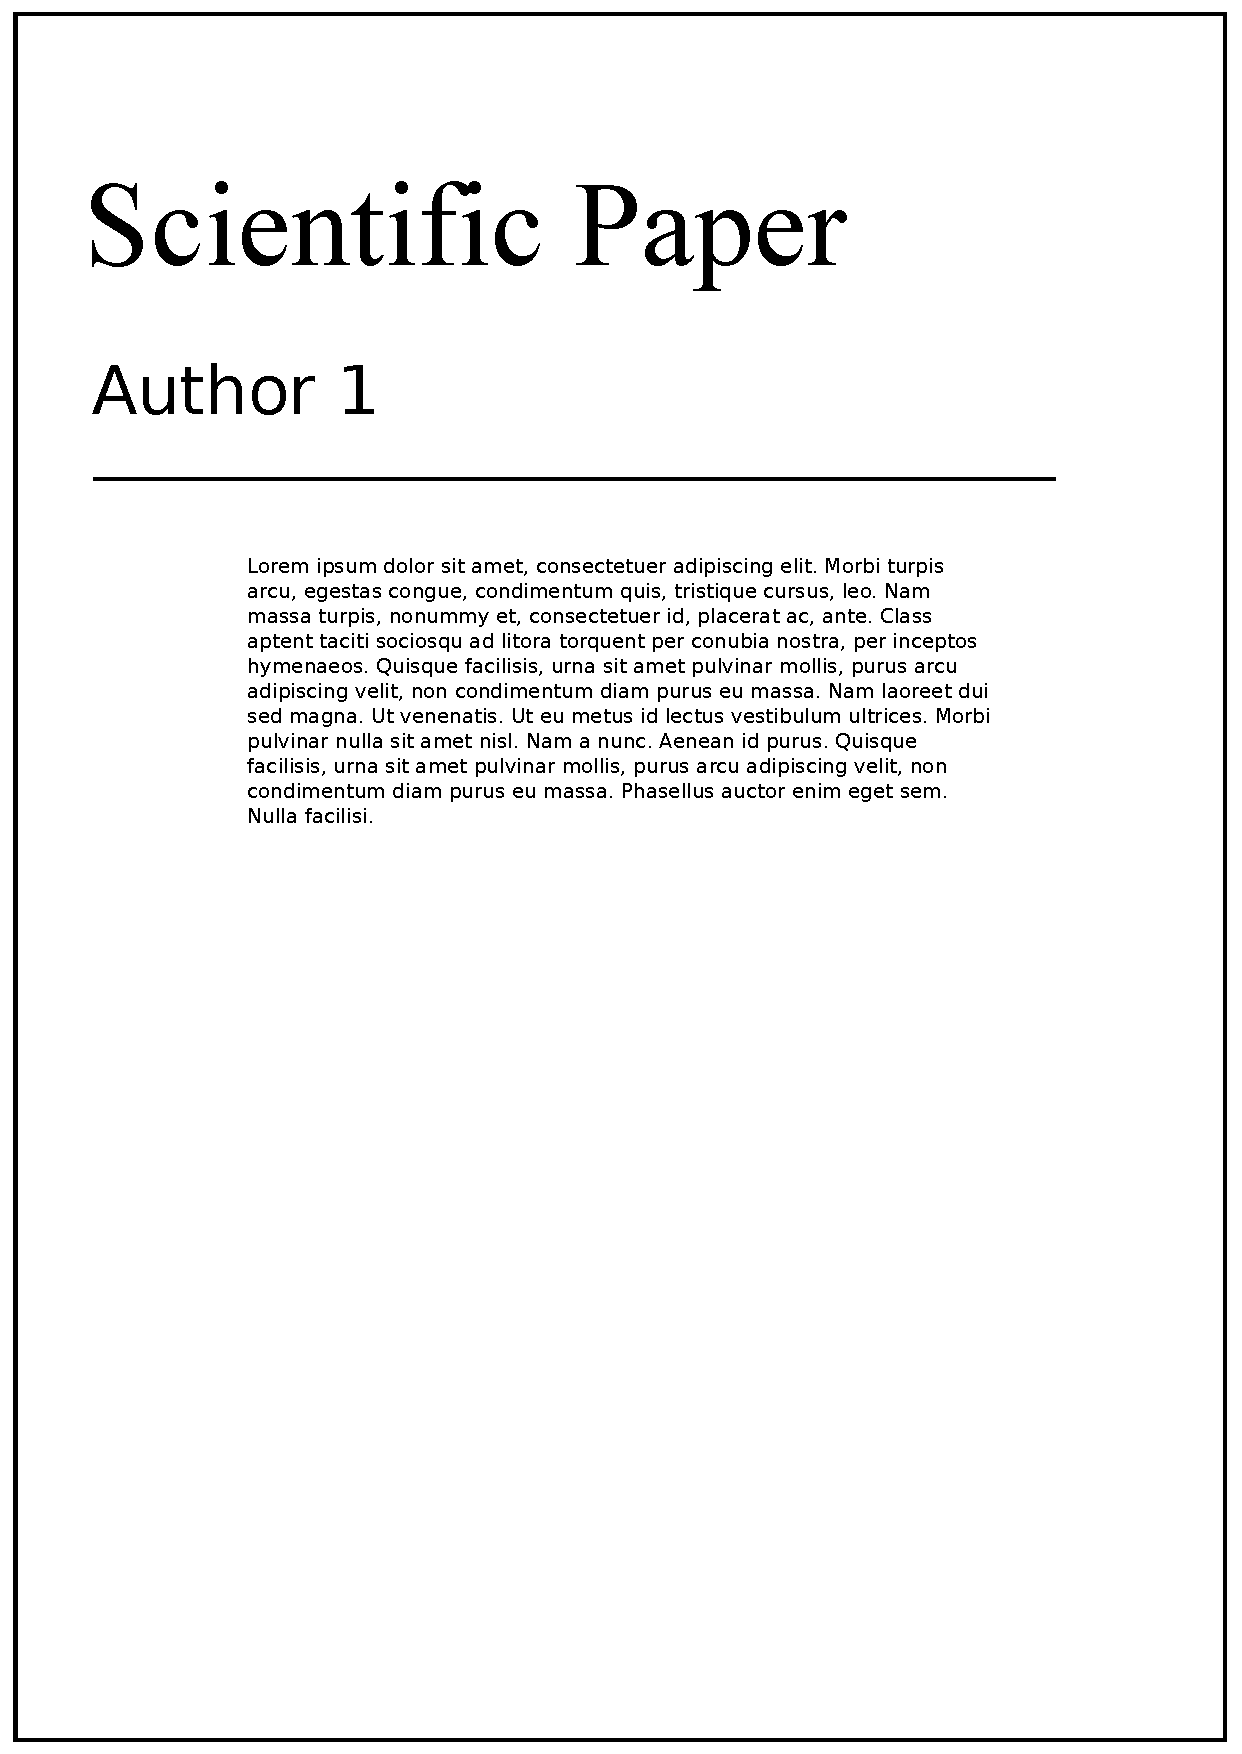
\includepdf[pagecommand=\thispagestyle{plain}, pages=-]{papers/paper1.pdf}

%****************************************************************
% Paper II
%****************************************************************
\renewcommand{\boxsizept}{52pt}
\chapter{Scientific Paper II}
\thispagestyle{empty}

\noindent List of authors\vspace{3ex}

\noindent \textit{In \Proc \IntlConf \ldots} \textbf{IEEE}, 035303 (2017)
\cleardoublepage
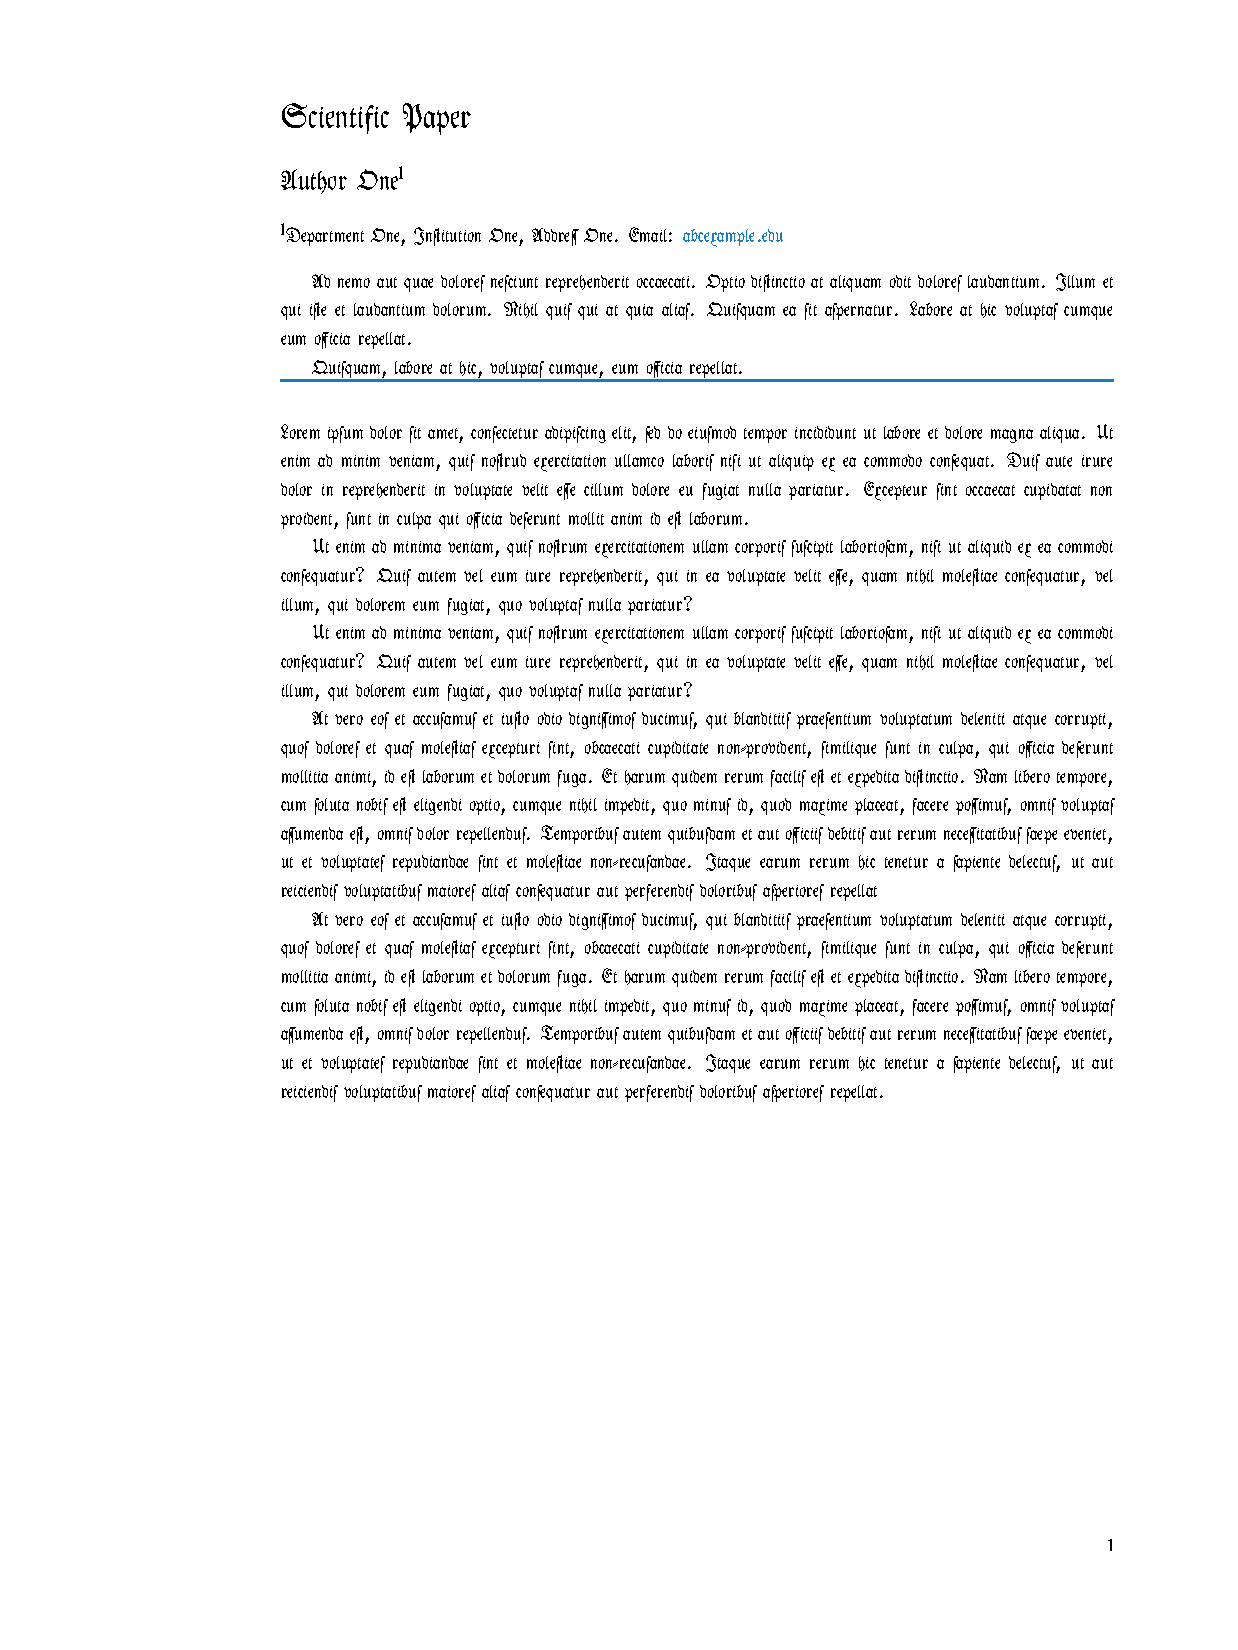
\includepdf[pagecommand=\thispagestyle{plain}, pages=-]{papers/paper2.pdf}

%****************************************************************
% Paper III
%****************************************************************
\renewcommand{\boxsizept}{56pt}
\chapter{Scientific Paper III}
\thispagestyle{empty}

\noindent List of authors\vspace{3ex}

\noindent \textit{In \Proc \IntlConf \ldots} \textbf{IEEE}, 035303 (2017)
\cleardoublepage


%****************************************************************
% Paper IV
%****************************************************************
\renewcommand{\boxsizept}{60pt}

\chapter{Scientific Paper IV}
\thispagestyle{empty}

\noindent List of authors\vspace{3ex}

\noindent \textit{In \Proc \IntlConf \ldots} \textbf{IEEE}, 035303 (2017)
\cleardoublepage

\pagestyle{compiledpapers} % if you use compiled papers with \subimport{}

% the subimport like below to find main.tex in your paper folder,
% the main.tex also needs to be modified to only have \input{} and other useful commands
% (better to make a backup first or make a new branch on you paper repository on Github)
\subimport*{papers/paperdummytex/}{main-dummy.tex}

  % The papers, with cover pages
\end{appendices}

%*******************************************************
% Backmatter
%*******************************************************
\newpage
\listoffigures

\let\cleardoublepage\clearpage

\newpage
\lstlistoflistings

\let\cleardoublepage\clearpage

\newpage
\listoftables

\backmatter
%*******************************************************
% Game Over
%*******************************************************
\end{document}
